
\chapter{RESULTS AND DISCUSSIONS}

\section{{\bf{Result}}}

For the purpose and verification by a concrete example and demonstration of potential application of the method, we designed a custom truss and studied its deformations under the prescribed forces . These forces and the overall structure of truss is as below.\\
\noindent

\begin{figure}[h]
	\centering
	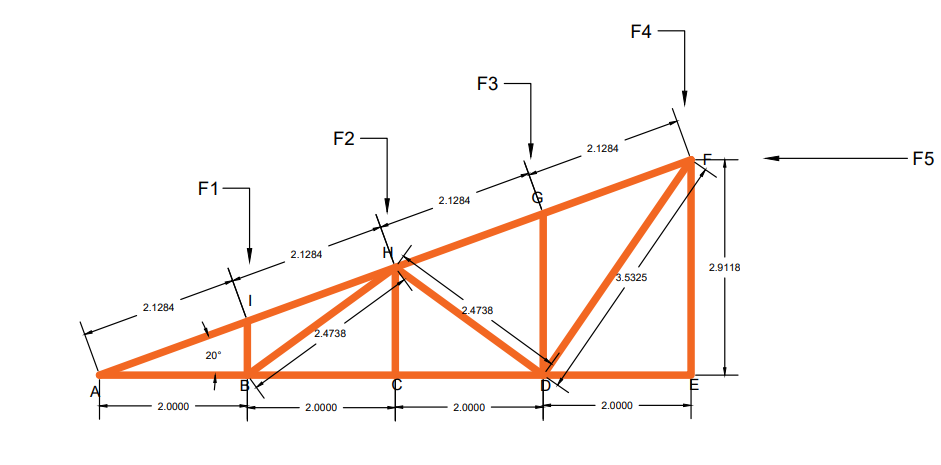
\includegraphics[width=0.8\linewidth , height=0.5\linewidth]{truss}
	\caption{Truss}
\end{figure}

\noindent

Our module drew the structure of truss as
\begin{figure}[h!]
	\centering
	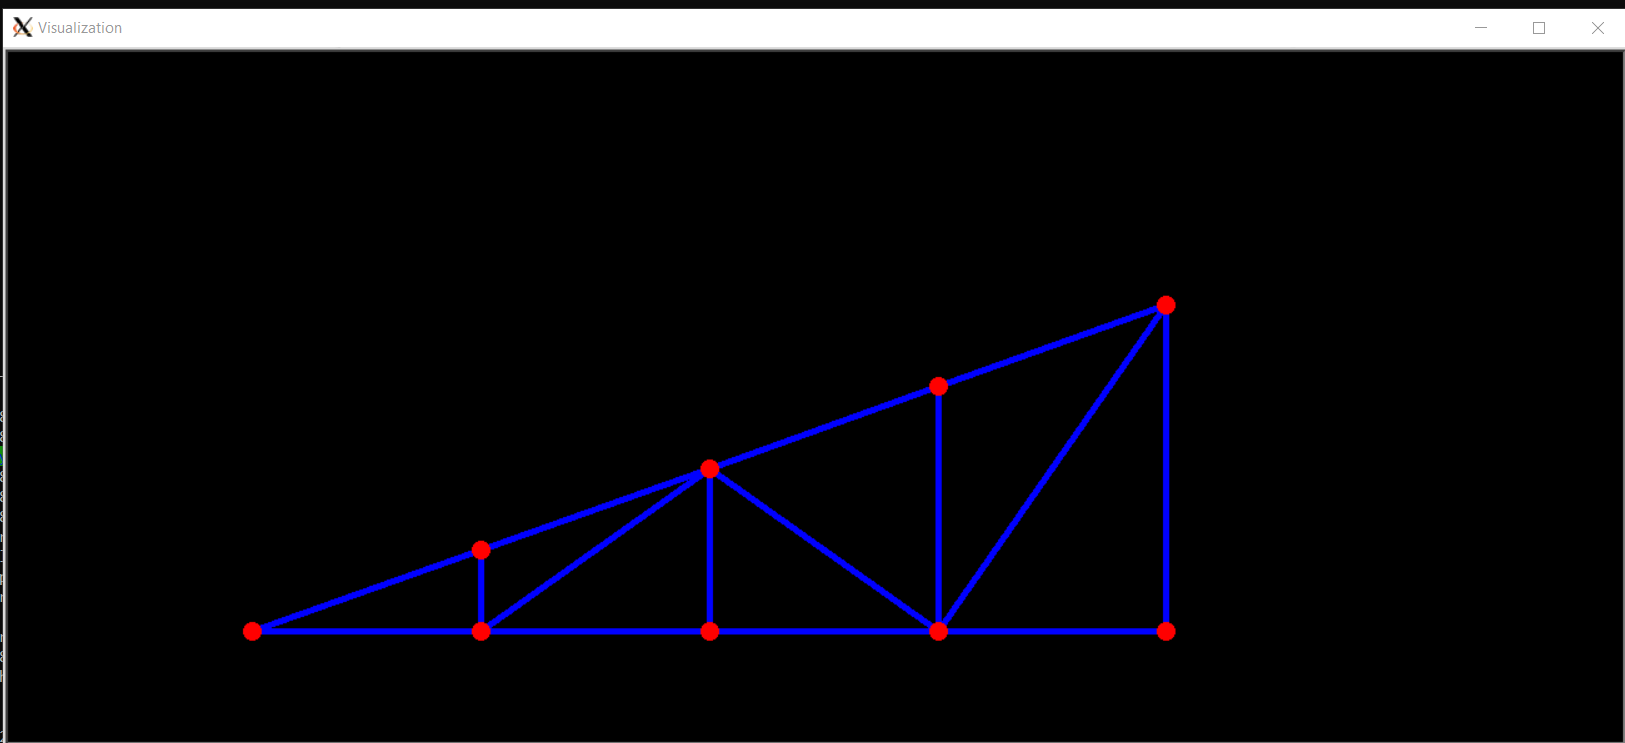
\includegraphics[width=0.8\linewidth , height=0.5\linewidth]{before}
	\caption{Above Truss as drawn by truss\_solve module}
\end{figure}

Implementing the problem in python gave the following structure after deformation.\\
\begin{figure}[h!]
	\centering
	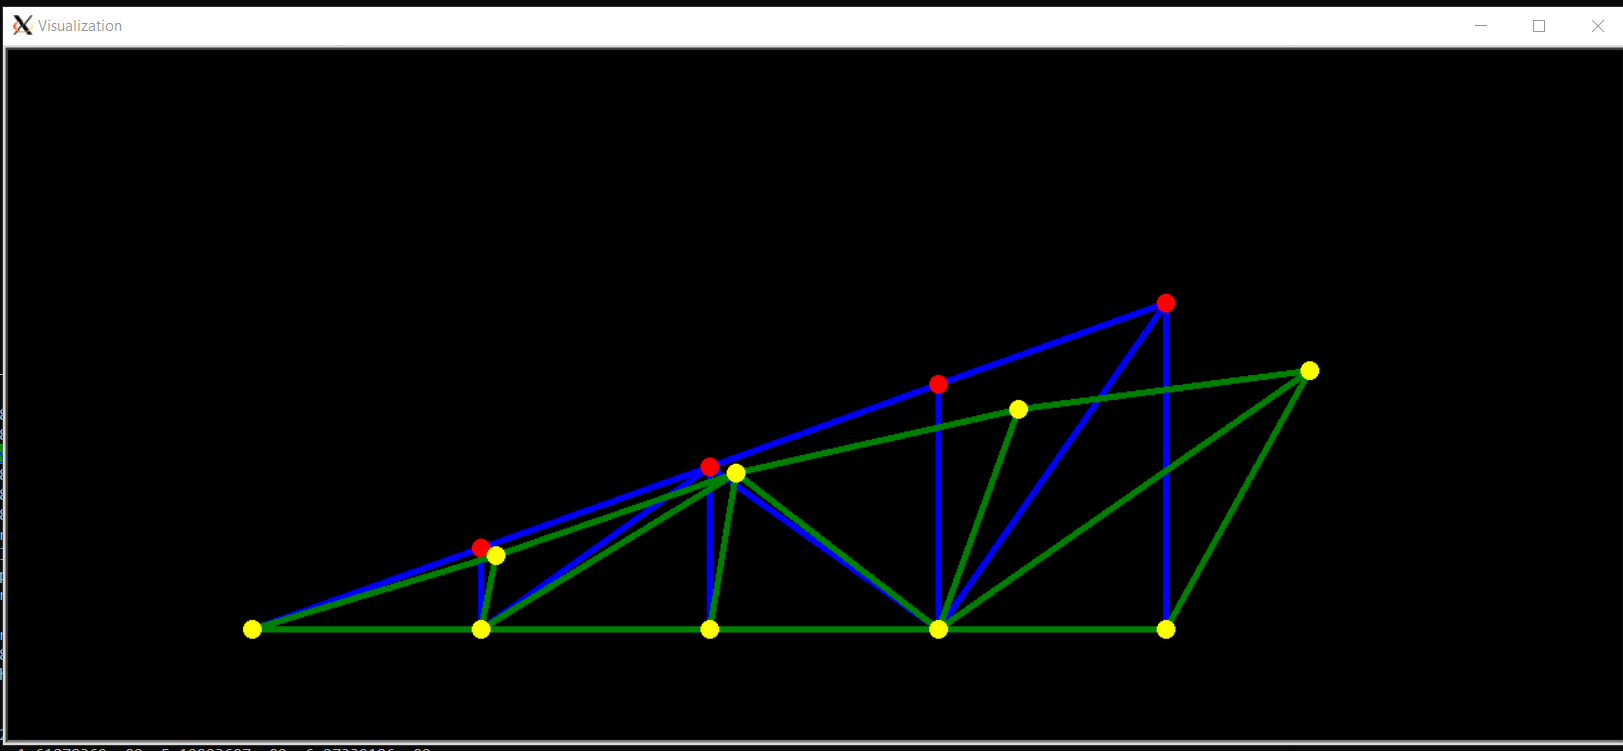
\includegraphics[width=0.8\linewidth , height=0.5\linewidth]{after}
	\caption{Above Truss along with deformation}
\end{figure}

%ss from jupyter notebook.   

\pagebreak
We also verified our solution in Frame3dd. Frame3dd is a free open-source software for static and dynamic structural analysis of 2D and 3D frames and trusses with elastic and geometric stiffness.  It is a copyright of
\begin{center}
     Department of Civil and Environmental Engineering\\
	Edmund T. Pratt School of Engineering\\
	Duke University - Box 90287, Durham, NC 27708-0287\\
	Henri P. Gavin, Ph.D., P.E.,
\end{center}
\begin{figure}[h!]
	\centering
	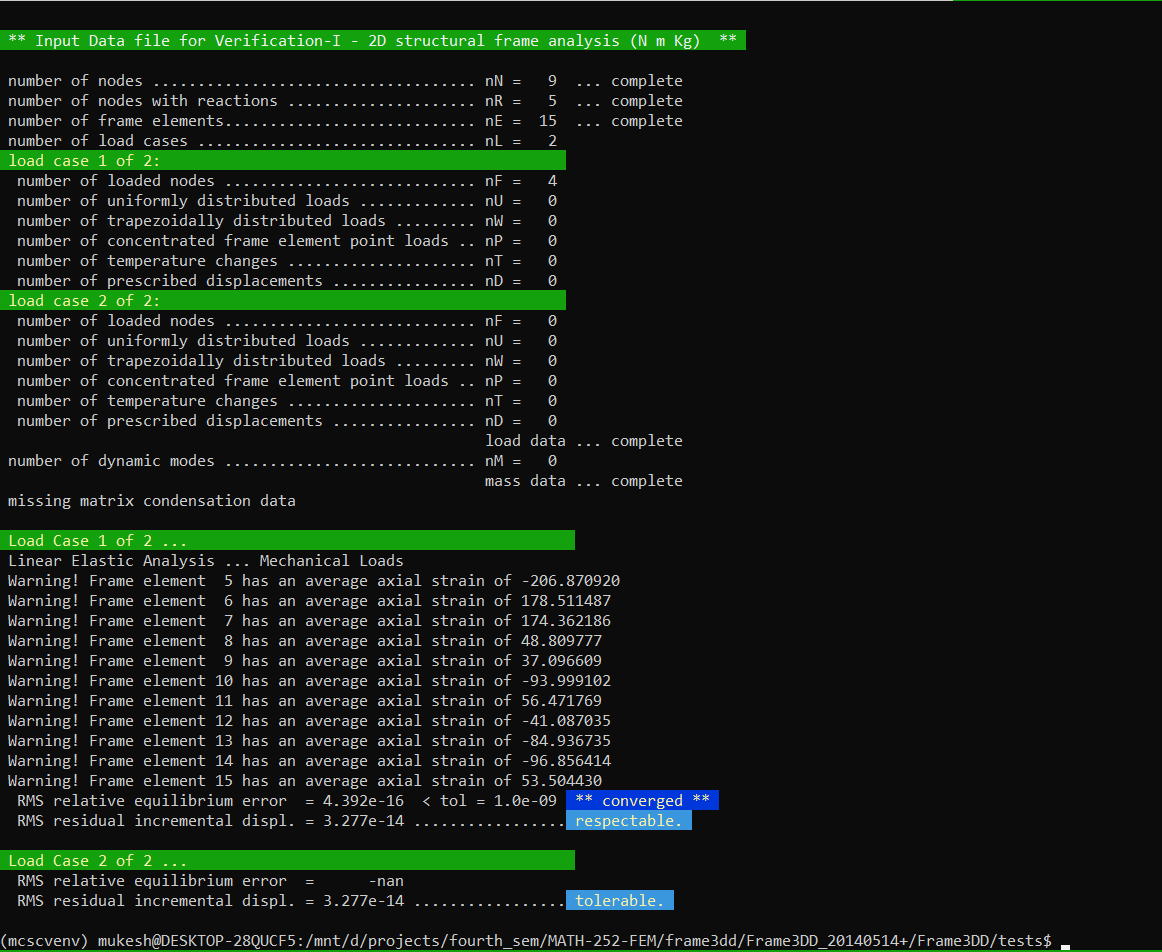
\includegraphics[width=0.8\linewidth , height=0.9\linewidth]{frame}
	\caption{Solving using Frame3DD}
\end{figure}

After verification in the software, the following structure was obtained.\\

%ss from fram3dd
\begin{table}[h!]
	\centering
	\begin{tabular}{|l|l|l|l|}
		\hline
	      Results in python & Results in frame3dd   \\
		\hline
	
	      12.48407187  &12.1552098            \\
	     -6.04631381   &-6.03649343           \\
	      7.00856832   & 6.66504758           \\
	     -2.1838       &-2.11534409           \\
	      2.35025907   & 2.16352748           \\
	     -0.56650909   &-0.59822723           \\
         -0.7279       &-0.68431346           \\
        
		\hline  
	\end{tabular}
		\caption{Comparision of results obtained in python to that in frame3dd for displacement.}
\label{Comparision_table}
\end{table}

Table \ref{Comparision_table} shows the percentage error in each node for displacement. Going from left to right we get  displacement a as obtained in python, displacement as obtained in frame3dd and percentage error in each displacement.\\

The average percentage error in displacement is $1.73 \% $.\\



